\section{The history of Ethernet and single segment}

Ethernet was developed at Xerox PARC in 1973 and commercially introduced in 1980 as the so-called "DIX" (Digital, Intel, Xerox) standard with a bandwidth of 10Mbit/s, using coaxial cables and described as a technology for local-area networks. Ethernet became dominant over Token Ring in the end of the 1980's, because Ethernet was more adaptive than these proprietary protocols and quickly switched to the twisted-pair wiring (UTP, unshielded twisted pair), reducing cost, complexity and boosting transmission rates.

\noindent The Ethernet standard was intended for a typical office environment with workstations, but did also support PC-based controllers, PLC's and other devices, because it was an open-standard and easily accessible. Figure \ref{fig:plantcontroldevice} illustrates a Plant-Control-Device environment, with higher response times at the plant level, more data transfers but less frequency.

\begin{figure}[h!]\label{}
	\centering
	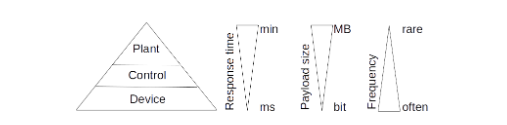
\includegraphics[scale=0.5]{realTimeEthernet/PlantControlDevice.png}
	\caption{The plant, control and device segments of a domain. Plant span entire facilities, control span plant floors and device span parts of plant floor.}
	\label{fig:plantcontroldevice}
\end{figure}

\noindent The first mid-80's Ethernet technologies (10BASE2, 10BASE5, and early 10BASE-T) constituted a so-called single segment network and relied on hubs, repeaters and the CSMA/CD (Carrier Sense Multiple Access with Collision Detection) protocol for sharing bandwidth on a shared medium. It was relatively low cost and flexible, but nondeterministic medium access made it hard to guarantee deadlines and use in a real-time system with no packet prioritization. Also speed was a function of the number of nodes on a network link. When sending, CSMA/CD implements carrier-sense by listening on the network for traffic. If it occurs, it does not transmit data. If no traffic for a certain period, it transmits data. Multiple Access allows more nodes to share the medium, but means collisions are more likely and that all packets are passed to all nodes. To mitigate this, the protocol brings Collision Detection, where a node listens for collisions on the medium, if they occur it sends a jam signal, back-offs for a random time period (exponential back-off algorithm) and tries again.

\noindent The truncated exponential back-off algorithm (EBA) retransmits after a random back-off time given by:

\[ T_{back-off}: r \times T_{slot} \]

\noindent with these properties:

\begin{itemize}
	\item $T_{slot}$ = $T_{dataout}$ + $T_{jam-back}$. The time it takes for the data to be sent to the point of collision and for the jam signal to get back. It is the max theoretical round-trip time.
	\item r $\sim$ \textit{u}[0, ..., 2\^{c} - 1], where \textit{u} is a uniform distribution.
	\item c is a local node counter, c $\in$ [1;$c_max$], and is reset after successful transmission. $c_max$ = 10 in the IEEE 802.3 CSMA/CD standard. Truncation means that after a certain number of increases, exponentiation stops and is reset.
\end{itemize}

\noindent For 10Mbit/s Ethernet, $T_{slot}$ = 51.2$\mu$s and decreases when transmission rates $\longrightarrow$ $\propto$. Figure \ref{fig:csmacd} shows a collision on the wire, how the two re-transmissions collide and the random back-off timer in effect.

\begin{figure}[H]\label{}
	\centering
	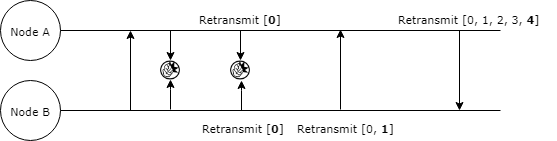
\includegraphics[scale=0.5]{realTimeEthernet/CSMACD.png}
	\caption{CSMA/CD in effect with random re-transmissions upon collisions.}
	\label{fig:csmacd}
\end{figure}
\noindent A conceivable drawback of the back-off algorithm is that it can introduce medium monopolization by one node in a network, $Node_{b}$, depriving another node, $Node_{a}$ of time to send. As the back-off algorithm is random, if $Node_{b}$ is more successful than $Node_{a}$ at sending packets, $Node_{a}$'s collision counter might increase beyond that of $Node_{b}$, resulting in exponential wait times for $Node_{a}$. In the next chapter we look at how to solve collisions using network segmentation.

